% Supplementary material for IEEE TTE submission (paper v8).
% Moved from the main manuscript to meet the TTE regular-paper length limit
% (target 6--8 pages; regular papers over 10 pages may be rejected).
\documentclass[journal]{IEEEtran}
\usepackage{amsmath,amssymb,booktabs,graphicx,multirow,siunitx,xcolor,cite}
\graphicspath{{figs/}}
\begin{document}
\title{Supplementary Material: Temperature-Parametrised Kalman Priors and Learned Corrections for Lithium-Ion State-of-Charge Estimation}
\author{Suyash~D.~Nahar\emph{et~al.}}
\maketitle
\begin{abstract}
Tables and one figure moved from the main manuscript for length. Numbering below matches the labels used in the main text (\texttt{tab:conv}, \texttt{tab:diag}, \texttt{tab:oracle}, \texttt{tab:aged}, \texttt{fig:tracking}).
\end{abstract}

\section{Convergence (Main Text Table~\ref*{tab:conv})}
\begin{table}[!t]
\caption{Convergence Time (Median, s; Minimum 30~s) and Share of Segments That Converge Into $\pm2$\% for 60~s}
\label{tab:conv}
\centering\scriptsize
\begin{tabular}{@{}lcccc@{}}
\toprule
 & \multicolumn{2}{c}{LG-L} & \multicolumn{2}{c}{S-L}\\
Estimator & Time & Share & Time & Share\\
\midrule
EKF & 103 & 86\% & 30 & 54\% \\
SPKF & 30 & 86\% & 30 & 58\% \\
SHEKF & 110 & 91\% & 30 & 58\% \\
BiLSTM & 30 & 86\% & 30 & 96\% \\
PI-LSTM & 30 & 91\% & 30 & 96\% \\
Fusion & 30 & 95\% & 30 & 83\% \\
LSTM & 30 & 91\% & 426 & 92\% \\
GRU & 762 & 82\% & 309 & 71\% \\
CNN-LSTM & 30 & 86\% & 286 & 83\% \\
LSTM+KF & 30 & 95\% & 547 & 92\% \\
\bottomrule

\end{tabular}
\end{table}

\section{SPKF Diagnostic (Main Text Table~\ref*{tab:diag})}
\begin{table}[!t]
\caption{SPKF Diagnostic, Legacy Versus Corrected Sigma-Point Scaling: Segments With Non-Positive-Definite $\mathbf{P}$ or Failed Cholesky, Mean Segment RMSE (\%), Segments With Maximum Error Above 20\%}
\label{tab:diag}
\centering\scriptsize
\begin{tabular}{@{}lccc@{}}
\toprule
Run and setting & Failures & Mean RMSE & $>$20\%\\
\midrule
LG-L, legacy & 0 of 63 & 1.77 & 21 \\
LG-L, corrected & 0 of 63 & 1.65 & 15 \\
S-L, legacy & 0 of 72 & 3.10 & 19 \\
S-L, corrected & 0 of 72 & 2.92 & 18 \\
LG-E, legacy & 0 of 53 & 3.30 & 17 \\
LG-E, corrected & 0 of 53 & 2.85 & 10 \\
S-E, legacy & 0 of 60 & 6.01 & 25 \\
S-E, corrected & 0 of 60 & 4.06 & 19 \\
\bottomrule

\end{tabular}
\end{table}

\section{Parameter Oracle (Main Text Table~\ref*{tab:oracle})}
\begin{table}[!t]
\caption{Parameter Oracle, LG-E: Test RMSE (\%) When One Extrapolated Quantity Is Replaced by Its Directly Identified Value (SHEKF Prior Run)}
\label{tab:oracle}
\centering\scriptsize
\begin{tabular}{@{}rlccc@{}}
\toprule
$T$ ($^\circ$C) & Variant & EKF & SPKF & SHEKF\\
\midrule
0 & Extrapolated (as used) & 2.78 & 2.57 & 3.31 \\
0 & $R_0$ direct & 2.13 & 1.99 & 2.61 \\
0 & $R_1$ direct & 2.73 & 2.53 & 3.27 \\
0 & Capacity direct & 2.76 & 2.56 & 3.29 \\
0 & OCV direct & 2.24 & 2.08 & 2.65 \\
0 & $R_0,R_1,\tau_1$ direct & 2.04 & 1.90 & 2.46 \\
0 & All direct & 1.81 & 1.65 & 1.88 \\
\midrule
-10 & Extrapolated (as used) & 5.11 & 4.44 & 5.64 \\
-10 & $R_0$ direct & 4.56 & 4.32 & 4.70 \\
-10 & $R_1$ direct & 5.62 & 4.90 & 6.01 \\
-10 & Capacity direct & 5.48 & 4.83 & 6.35 \\
-10 & OCV direct & 5.57 & 4.33 & 5.65 \\
-10 & $R_0,R_1,\tau_1$ direct & 4.53 & 4.04 & 4.58 \\
-10 & All direct & 4.53 & 4.03 & 4.90 \\
\midrule
-20 & Extrapolated (as used) & 10.62 & 10.30 & 10.88 \\
-20 & $R_0$ direct & 13.45 & 13.09 & 12.95 \\
-20 & $R_1$ direct & 11.88 & 11.15 & 11.37 \\
-20 & Capacity direct & 9.91 & 9.21 & 10.53 \\
-20 & OCV direct & 10.86 & 10.53 & 11.72 \\
-20 & $R_0,R_1,\tau_1$ direct & 10.24 & 10.05 & 9.90 \\
-20 & All direct & 10.31 & 10.16 & 10.65 \\
\bottomrule

\end{tabular}
\end{table}

\section{Aged-Cell Transfer (Main Text Table~\ref*{tab:aged})}
\begin{table}[!t]
\caption{Braun: Fresh-Cell Test RMSE and Aged-Cell Transfer (\%), Nothing Refitted. Left Block: B-W Models; Right Block: B-R Models (SHEKF Prior)}
\label{tab:aged}
\centering\scriptsize
\begin{tabular}{@{}lcccccccc@{}}
\toprule
 & \multicolumn{4}{c}{B-W} & \multicolumn{4}{c}{B-R}\\
 Estimator & Fresh & Aged & MAE & Max & Fresh & Aged & MAE & Max\\
\midrule
EKF & 4.14 & 1.66 & 1.33 & 3.98 & 3.74 & 1.66 & 1.33 & 3.94 \\
SPKF & 4.14 & 1.66 & 1.33 & 3.98 & 3.74 & 1.66 & 1.33 & 3.94 \\
IEKF & 4.14 & 1.66 & 1.33 & 3.98 & 3.74 & 1.66 & 1.33 & 3.94 \\
SHEKF & 4.32 & 2.33 & 1.81 & 6.30 & 3.95 & 2.30 & 1.79 & 6.20 \\
\midrule
LSBoost & 3.52 & 4.03 & 3.64 & 15.51 & 4.56 & 8.86 & 8.21 & 21.35 \\
PI-LSTM & 2.29 & 4.08 & 3.58 & 11.14 & 1.53 & 4.20 & 3.69 & 11.65 \\
BiLSTM & 3.49 & 4.99 & 3.90 & 17.05 & 3.96 & 2.62 & 2.11 & 7.52 \\
\midrule
NNLS fusion & 2.39 & 4.07 & 3.59 & 10.69 & 3.43 & 1.89 & 1.55 & 4.29 \\
\bottomrule

\end{tabular}
\end{table}

\section{Tracking Figure (Main Text Fig.~\ref*{fig:tracking})}
\begin{figure*}[!t]
\centering
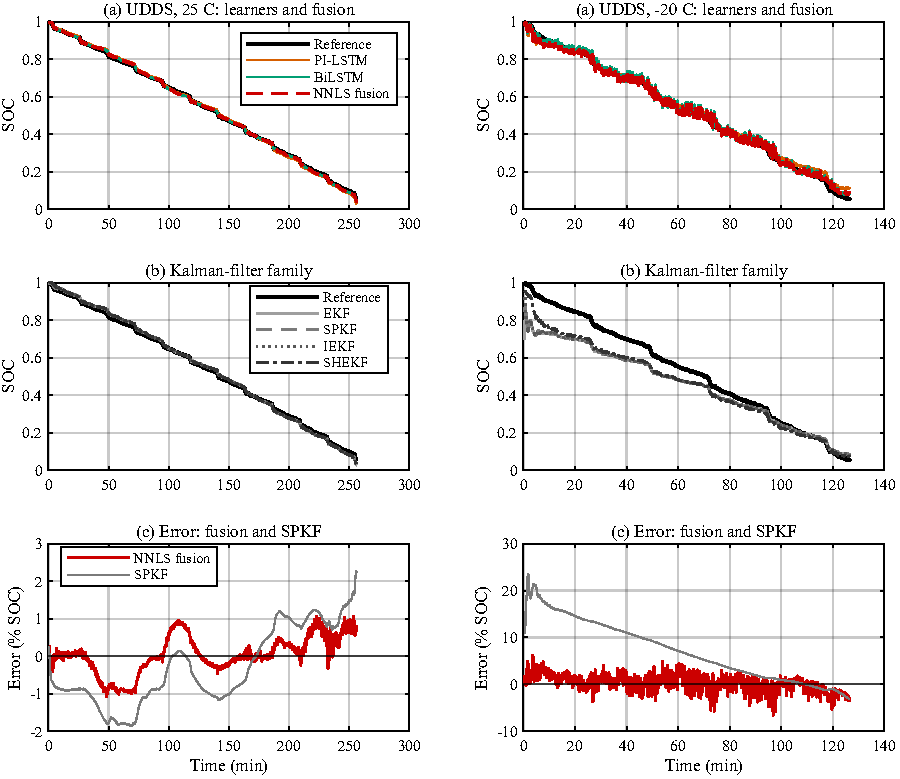
\includegraphics[width=\textwidth]{figs/v8_tracking_matlab.pdf}
\caption{LG-L: SOC tracking on UDDS at $25$~$^\circ$C (left) and $-20$~$^\circ$C (right), starting from a wrong initial SOC: (a) learners and fusion, (b) filters, (c) error of the fusion and the SPKF. At $-20$~$^\circ$C the filters keep an offset for the whole record.}
\label{fig:tracking}
\end{figure*}

\end{document}
